%*******************************************************************************
%****************************** Second Chapter *********************************
%*******************************************************************************

\chapter{The Prototype Detector}\label{Chp:ThePrototypeDetector}

\ifpdf
    \graphicspath{{Chapter2/Figs/Raster/}{Chapter2/Figs/PDF/}{Chapter2/Figs/}}
\else
    \graphicspath{{Chapter2/Figs/Vector/}{Chapter2/Figs/}}
\fi

\section{Technology And Results}
This thesis will cover two distinct versions of the detector. The original prototype detector was repurposed technology from the T2K ND280 ECal \cite{Allan_2013} and an upgraded version that uses the same basic materials in the detector but upgraded electronics and containment which will be referred to as the VIDARR detector. The rest of this section will focus on the prototype detector.
\\\\As it is the basis for the other detectors a quick overview of the T2K ND280 ECal will be required. The ND280 is a series of detectors from the neutrino oscillation experiment T2K which relies on a $\nu_\mu$ beam entering the detector shown in figure \ref{fig:nd280Fig}. This detector was comprised of several different detectors including time projection chambers (TPCs) and fine-grained detectors (FGDs) and electromagnetic calorimeters (ECals) \cite{Allan_2013}. The ECals are of particular interest as they are the basis for the prototype and VIDARR detectors. 

\begin{figure}[htbp]
 \centering
 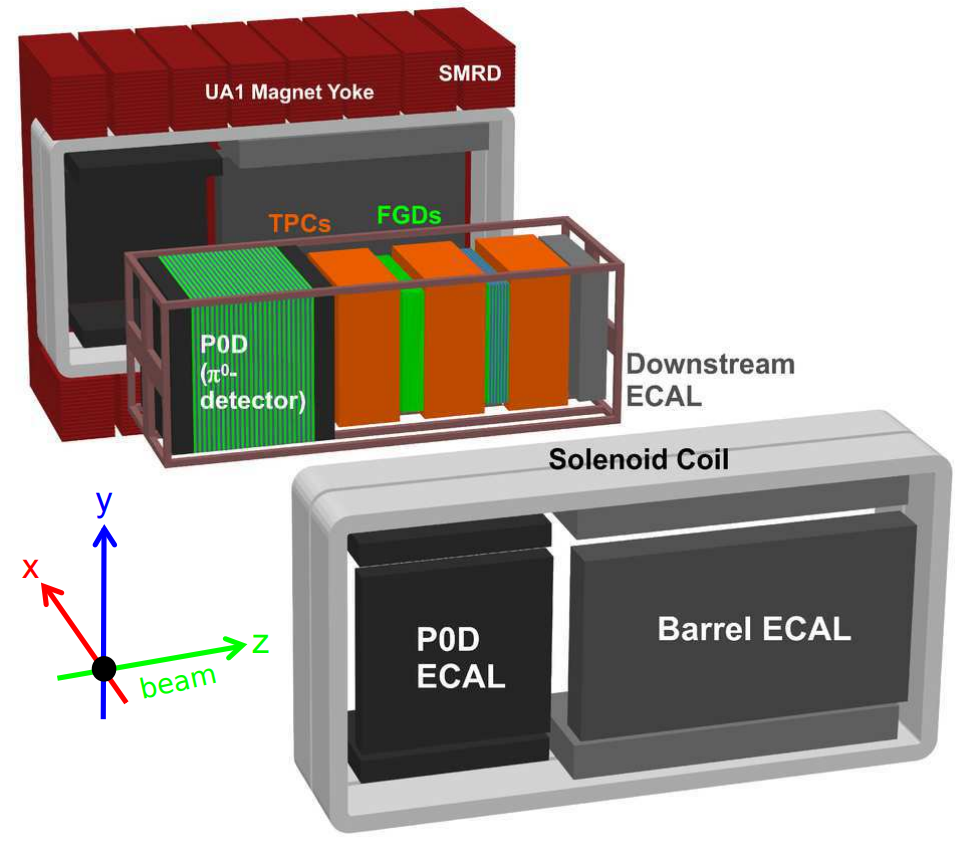
\includegraphics[width=\linewidth/2]{Chapter2/Figs/Raster/ND280Fig.png} 
 \captionof{figure}{Diagram of the ND280 detector. From \cite{Allan_2013}} %~can be used as a kind of place holder in latex
 \label{fig:nd280Fig}
\end{figure}

The T2K Ecals were made from plastic scintillating bars measuring 4\,cm by 1\,cm with varying lengths arranged in alternating layers at 90 degrees to each other \cite{Allan_2013}. Wavelength shifting (WLS) fibres were placed in the centre of the scintillating bars which shift the wavelength from blue to green \cite{Allan_2013}. These wavelength shifting fibres are then connected to multi-pixel photon counters (MPPCs) which are the instruments that read out the signal. This signal is then read in by Trip-T front-end electronic boards (TFBs) which then splits the signal into different cycles each containing 1.5 microseconds of information. All of this is shared by the prototype detector. 
\\\\However, a crucial difference between the ECals of the ND280 and the prototype detector is that the (ECals) had a layer of lead in between each of the plastic scintillating layers \cite{Allan_2013}. In the prototype, this has been replaced with a layer of gadolinium sulphate so that neutrons produced in IBD (equation \ref{inverse_beta_decay}) are captured. The prototype was also designed to fit inside of a shipping container each bar having a length of 152\,cm and the whole detector measuring 152\,cm by 152\,cm with 49 layers of plastic scintillating bars giving a height of 49\,cm and a total of 1862 bars. The electronic systems were also adapted from the T2K ECal. However, they were altered such that they were triggered from a neutron-induced gadolinium cascade from IBD. There were 23 cycles numbered from 0 -- 22 with 0 -- 17 cycles being considered "prompt" and cycle 18 being the trigger cycle. Cycles 19 -- 22 were left alone so that they could be compared in case time-dependent issues arose from the altered system. As will be discussed later in chapter \ref{chp:cosmicMuonTomography} these cycles were used to diagnose a time dependant issue with the cosmic $\mu$ data set.
\\The overall structure for the detector can be seen in figure \ref{fig:vidarrDiagram} where the orientation of the segments and how the WLS fibres shift protrude out of the ends is shown. In-between the layers of plastic there are layers of Gadolinium which absorb the neutrons from inverse $\beta$ decay shown in figure \ref{fig:inverse_beta_diagram}. The $\Bar{\nu_e}$ will be absorbed by a proton and decay into a $e^+$ and a neutron as shown in figure \ref{fig:inverse_beta_diagram}. The e$^+$ will decay producing two $\gamma$ rays which could be useful in distinguishing the e$^+$ from the general e$^-$ background. The neutron shown in figure \ref{fig:inverse_beta_diagram} is absorbed by the Gadolinium sheets in the detector which then causes an 8\,MeV $\gamma$ cascade which will be expanded upon in section \ref{sec:GEANT4Simulation_modellingGadolinium}.  

\begin{figure}[htbp]
 \centering
 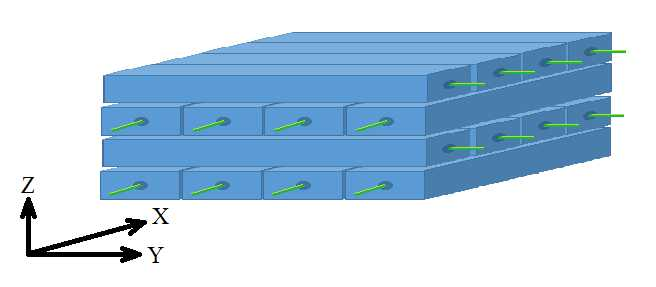
\includegraphics[width=0.8\linewidth]{Chapter2/Figs/Raster/VIDARR_diagram.jpeg} 
 \captionof{figure}{A cutaway diagram showing the structure of the VIDARR detector. The segments are 4\,cm wide by 152\,cm long by 1\,cm tall. The Gadolinium sheets in-between the VIDARR segments are not shown. (diagram created by George Holt fellow VIDARR collaborator).} 
 \label{fig:vidarrDiagram}
\end{figure}

\begin{figure}[htbp]
 \centering
 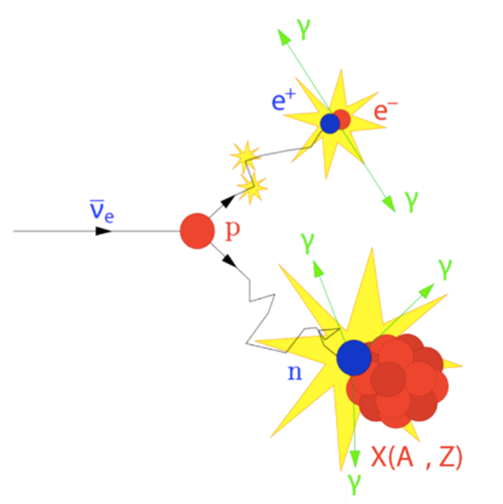
\includegraphics[width =0.7\linewidth]{Chapter2/Figs/Raster/inverse_beta_diagram.png}
 \captionof{figure}{A diagram of inverse $\beta$ decay 
 (equation \ref{inverse_beta_decay}). The neutrons random walk means it will take some time before it is detected the positron emission is prompt. From \cite{ibdPictureLink}.} 
 \label{fig:inverse_beta_diagram}
\end{figure}

The original detector was deployed at the Wylfa power station in Anglesey Wales for an 18-month period. This run proved successful in measuring the power from the reactor to within good agreement of the measured reactor flux. Figure \ref{fig:prototypeMeasumentFlux} compares the measured $\bar{\nu_e}$ flux with the reported power output and shows how good the agreement is. A measured anti-neutrino rate of 172.1 $\pm$ 4.6 candidates per day is observed when the reactor is off and 203.7 $\pm$ 19.6 when the reactor is on \cite{Carroll_2018}. Unfortunately due to cooling issues with the prototype detector the reactor shutdown was not observed. This is one of the main motivating factors behind the upgrade of the detector as the first generation MPPCs and repurposed electronics were susceptible to high levels of noise if the temperature was not carefully controlled. 
\begin{figure}[htbp]
 \centering
 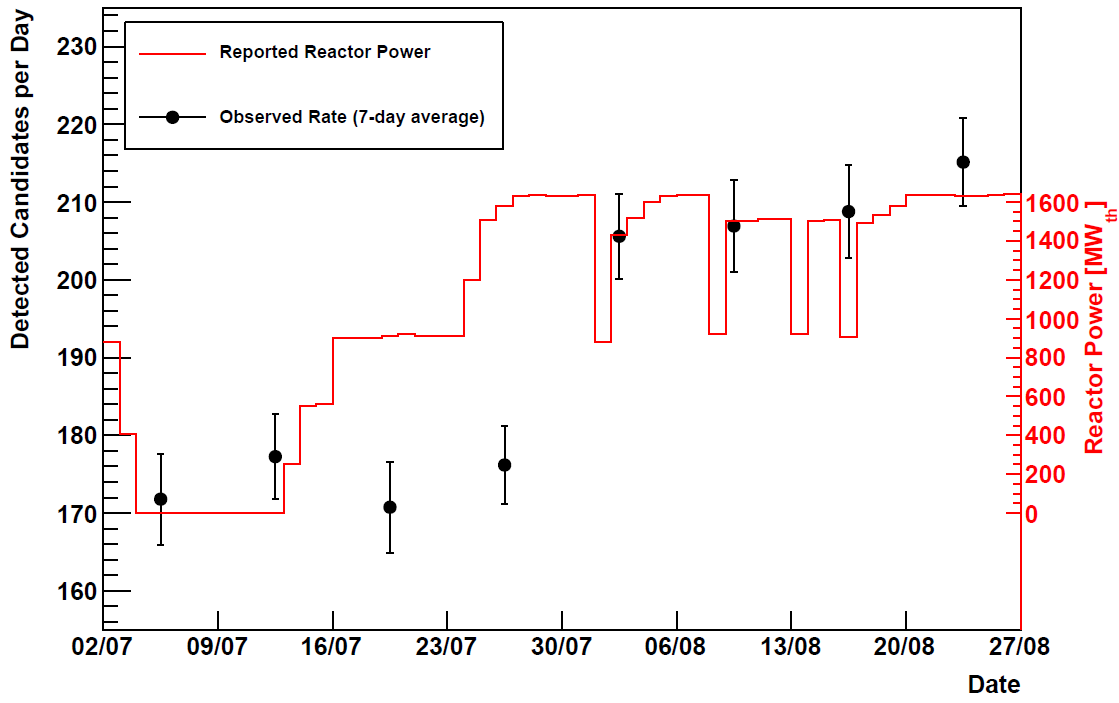
\includegraphics[width=0.90\linewidth]{Chapter2/Figs/Raster/prototypeMeasureOnFig.png} 
 \captionof{figure}{Measured anti-neutrino flux compared to the power generation from the Wylfa power station. From \cite{Carroll_2018}} %~can be used as a kind of place holder in latex
 \label{fig:prototypeMeasumentFlux}
\end{figure}

\section{Existing Reactor monitoring programs}\label{sec:exisitingReactorMonitoringPrograms}
%I feel like Double Chooz, Reno, KamLAND and Daya Bay are all very similar, liquid scintillating detectors with Gd doping initlally trying to find theta_13 but then transitioned to the 5 MeV reactor bump all of these are not proliforation focussed but measrument focussed experiments 
%Double Chooz is probably one of the most well known reactor monitoring programs. \cite{abe2014improved} goes over some of the details and I have already mentioned it here. Also the \cite{lasserre2006} reference may be useful, used it once before in the first year literature survey. I've also cited \cite{Abe_2012} in the past and that may prove useful here. Further the reference \cite{Olive_2014} may also be of use. Double Chooz is a good one to cite because its clearly not in competition with VIDARR. It requires to be very close and a big hole dug underground and uses gadolinium suspended in liquid organic scintillator. Which is not cheap or portable, it does however give significantly better measurements for the disappearance of anti-neutrinos which the above references mention.
The Double Chooz experiment is an evolution of the original Chooz experiment which was set up at the Chooz nuclear power plant in France\cite{lasserre2006}. Both of these experiments attempted to measure the $\Bar{\nu_e}$ disappearance from the same reactor however the original Chooz experiment was unable to see any disappearance to a 90$\,\%$ confidence level \cite{Apollonio_2003}. Both experiments used gadolinium doped liquid scintillator with the Double Chooz experiment having a near and far detector at 280\,m and 1050\,m respectively\cite{lasserre2006}. Finally, in 2012 $\Bar{\nu_e}$ disappearance was observed at the Double Chooz experiment \cite{Abe_2012}. These results were improved further in 2014 \cite{abe2014improved}.
\begin{figure}[htbp]
 \centering
 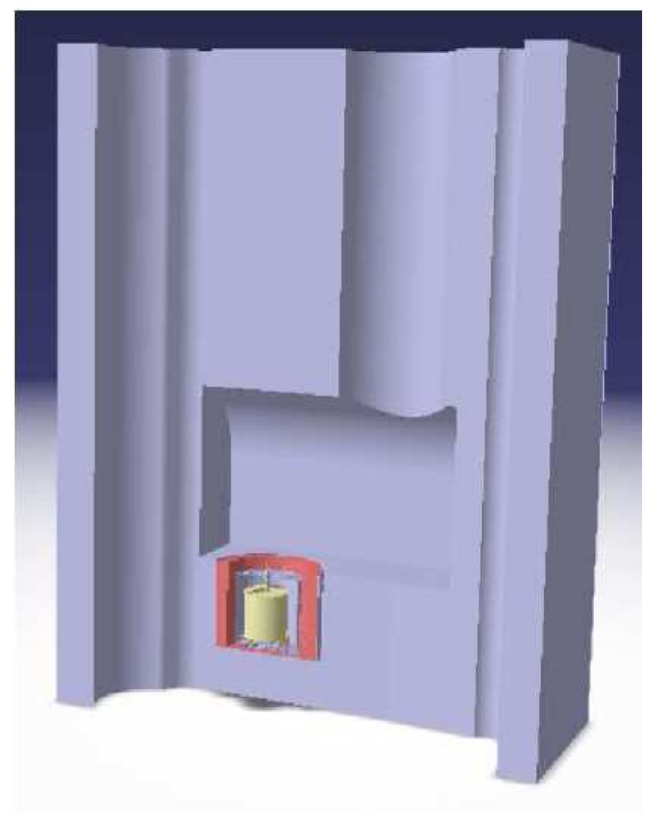
\includegraphics[height=75mm]{Chapter2/Figs/Raster/DCNearDetector.png} %height of this plot had to be adjusted because of its unusal diemensions
 \captionof{figure}{The near detector of the Double Chooz experiment 250\,m - 300\,m from the reactor with an overburden of 30\,m of rock. From \cite{lasserre2006}.} %~can be used as a kind of place holder in latex
 \label{DoubleChoozNearDetector}
\end{figure}
\\\\The Double Chooz experiment uses a detector placed underground to allow for a large amount of overburden to reduce background rates. As seen in figure \ref{DoubleChoozNearDetector} the overburden for the near detector is 30\,m\cite{lasserre2006}. The Double Chooz measurement  was not the first to measure the rate of $\Bar{\nu_e}$ disappearance \cite{reno_may_2012} it was able to produce a spectrum of the $\Bar{\nu_e}$ disappearance for $\theta_{13}$ which can be seen in \ref{doubleChoozSpectrumNoCaption}. The measured energy spectrum which can be seen as black points in figure \ref{doubleChoozSpectrumNoCaption}, the closest match to the data in the double Chooz data was found to the fitted red line with a $\sin^2{2\theta_{13}}$ = 0.109 $\pm$0.030(stat)$\pm$0.025(syst) as seen in figure \ref{doubleChoozSpectrumNoCaption} \cite{Abe_2012}. The data exclude the no-oscillation hypothesis at 99.8$\%$ CL (2.9$\sigma$)\cite{Abe_2012}. This data was further expanded upon in 2014 producing a result of $\sin^2{2\theta_{13}}$ = 0.090$^{+0.032}_{-0.029}$ using 467.90 live days of data to within $3.0\sigma$ \cite{abe2014improved}.
\begin{figure}[htbp]
 \centering
 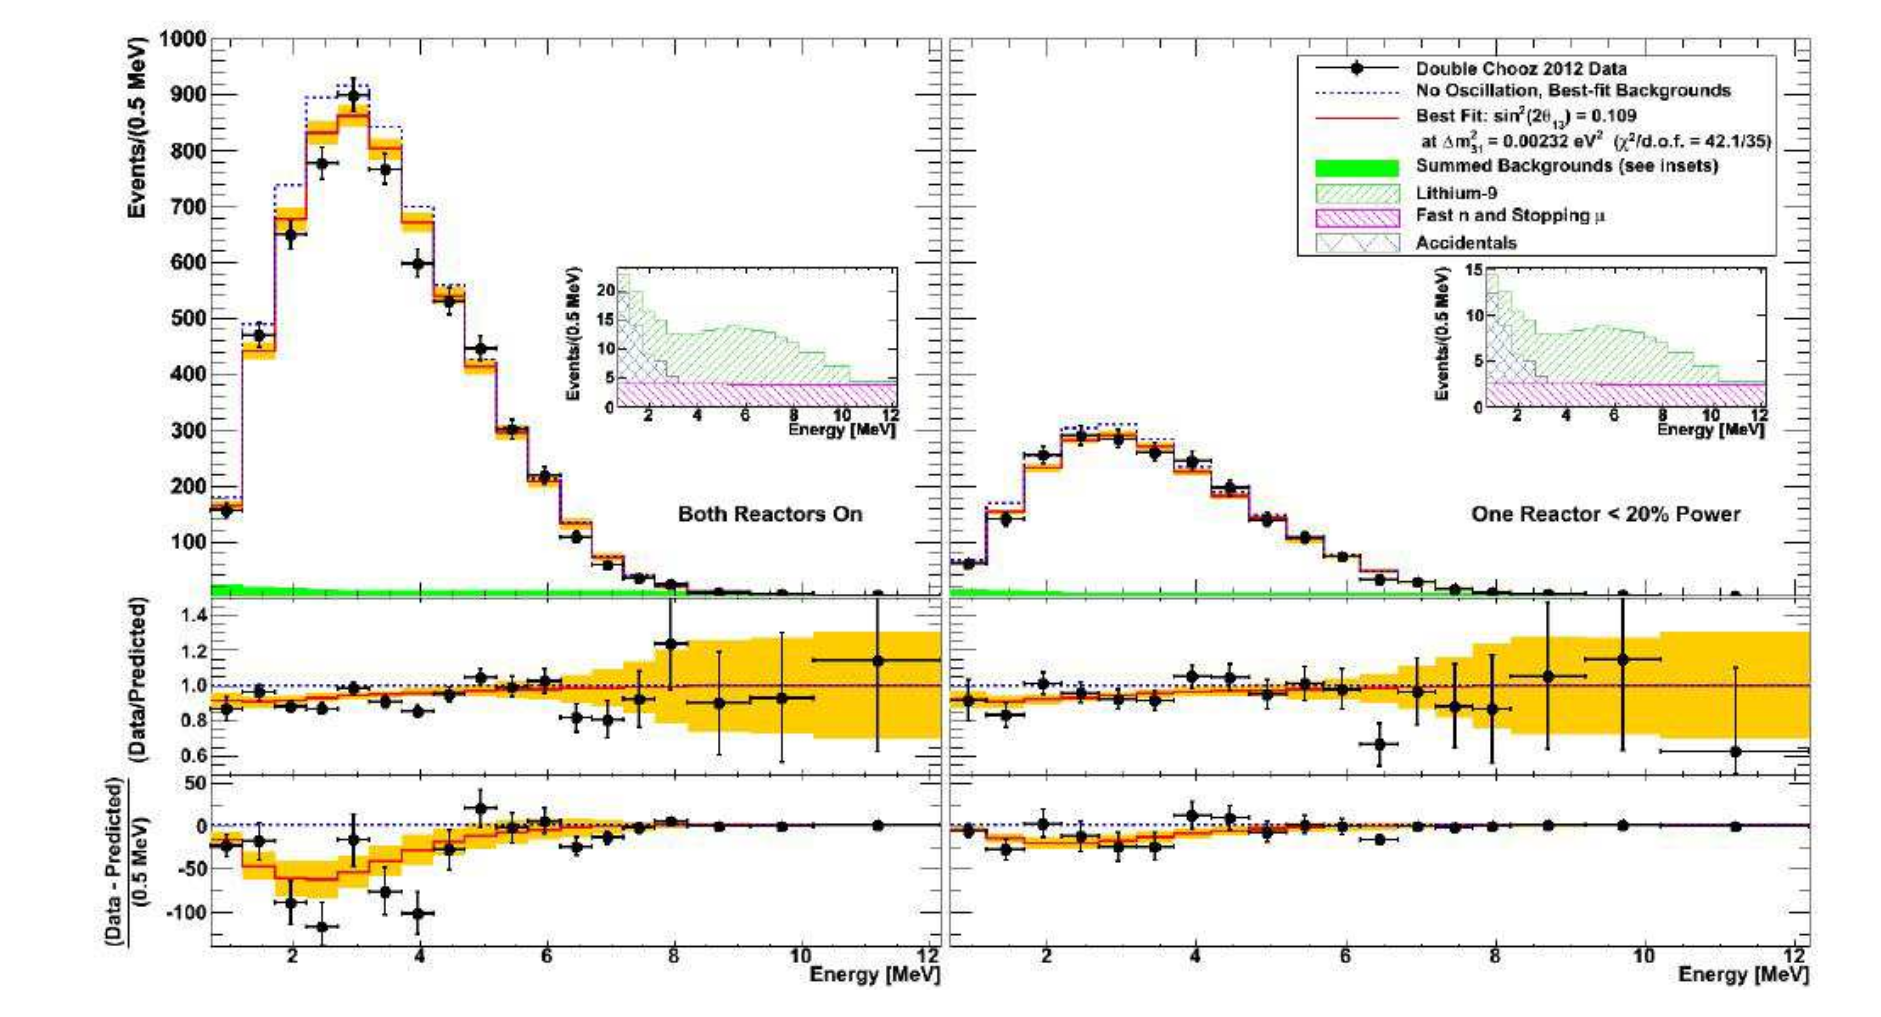
\includegraphics[width=\linewidth]{Chapter2/Figs/Raster/doubleChoozSpectrumNoCaption.png} %Just use linewidth for this one
 \captionof{figure}{Measured prompt energy spectrum for each integration period (data points) superimposed on the expected prompt energy spectrum, including backgrounds (green region), for the no-oscillation (blue dotted curve) and best-fit (red solid curve) at $\sin^2{2\theta_{13}}$ = 0.109 and $\Delta$m$^2_{31}$ = 2.32$\times$10$^{-3}$eV$^2$. Inset: stacked spectra of backgrounds. Bottom: differences between data and no-oscillation prediction (data points), and differences between best fit prediction and no-oscillation prediction (red curve).The orange band represents the systematic uncertainties on the best-fit prediction. From \cite{Abe_2012}} %~can be used as a kind of place holder in latex
 \label{doubleChoozSpectrumNoCaption}
\end{figure}

Papers found by this collaboration include \cite{reno_may_2012}, \cite{reno2013},  \cite{reno_may_2019}. Reno was the first collaboration to see $\Bar{\nu_e}$ disappearance \cite{Olive_2014}. The RENO experiment consisted of two detectors 408.56\,m for the near detector, and 1443.99\,m for the far detector. A schematic of the detectors used in RENO can be seen in figure \ref{RENO_detector}, this detection system again uses Gd-doped liquid scintillator with PMTs. 

\begin{figure}[htbp]
 \centering
 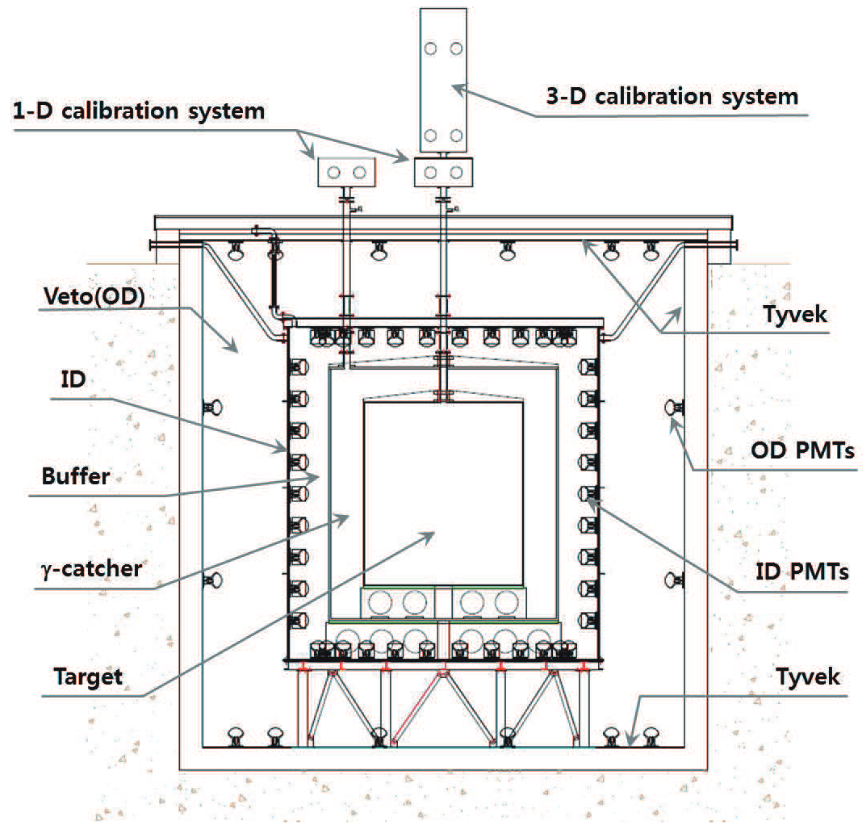
\includegraphics[width=0.5\linewidth]{Chapter2/Figs/Raster/RENO_detector.png} %Just use linewidth for this one
 \captionof{figure}{ schematic view of a RENO detector. The near and far detectors are identical. The detector seen in this figure consists of a main inner detector (ID) and an outer veto detector (OD) from \cite{reno_may_2012}} %~can be used as a kind of place holder in latex
 \label{RENO_detector}
\end{figure}

RENO's results in 2012 were consistent with neutrino oscillations to within 4.9 $\sigma$ from 6 2.8\,$GW_{th}$ reactors. The result from RENO in 2012 using a rate based analysis was $\sin^2{2\theta_{13}}$ = 0.113$\pm0.013$(stat.)$\pm0.019$(syst.) which was consistent with the findings that Double Chooz would produce later. These results were revised once again in 2013 using 800 days of live time to $\sin^2{2\theta_{13}}$ = 0.100 $\pm$ 0.010(stat) $\pm$ 0.015 (sys.) corresponding to 6.3 $\sigma$ significance \cite{reno2013}. The focus of the RENO collaboration has since shifted to analysing the 5\,MeV reactor anomaly \cite{reno_may_2019}.  
\\\\There are similar experiments to both Double Chooz and RENO. For example, the Daya Bay experiment in China uses similar technology to measure anti-neutrinos from reactors \cite{DayaBay2007Precision}. Similar to other experiments in this field the Daya Bay experiment has started to measure the reactor anomaly at 5\,MeV \cite{Daya_Bay_2017}. Nucifer is also similar to the other experiments being a scaled-down version of Double Chooz, Daya Bay and RENO using Gd doped liquid scintillator with the goal of near field reactor monitoring \cite{nucifer2016}. Another experiment of interest is the WATCHMAN collaboration which has the goal of far-field reactor monitoring using $\bar{\nu_e}$ originally planned to be deployed in the U.S.A \cite{askins2015physics} it has since become a joint U.S, U.K project and will be deployed at Boulby mine \cite{burns2018remote} its technology is in a state of flux but will use Gd in a fluid detector. There has been some external collaboration between the VIDARR experiment and the WATCHMAN experiment. In particular the application of the DANCE calorimeter data to form a dice box for Gadolinium which VIDARR has also taken advantage of. % There is another paper for WATCHMAN talking about directionallity but this is a bit of a can of worms... \cite{danielson2019directionally} 
\\\\Whilst the previously mentioned experiments are a useful context for the VIDARR detector their goals and technology differ. The following experiments of PANDA, SoLid, and to some extent CHANDLER are more comparable. This is because they are solid plastic scintillators aiming for deployments at commercial reactor sites (at least for PANDA and SoLid). As such it is useful to see the compromises that these experiments have made in comparison to VIDARR. The Plastic Anti-Neutrino Detector Array (PANDA) is a segmented detector that uses plastic and Gadolinium shown in figure \ref{subFig:pandaClose}, the gadolinium's interaction with neutrons is shown in equation \ref{equ:gadolinumNAbsorption}. The bars clustered together can be seen in figure \ref{subFig:pandaFar}. The bars seen in figure \ref{subFig:pandaFar} are plastic scintillator with dimensions of 10\,cm $\times$ 10\,cm $\times$ 100\,cm with two 10\,cm\ $\times$ 10\,cm $\times$ 10\,cm acrylic cubic light guides are glued to both ends of the plastic scintillator with optical cement capped with photon multiplier tubes at either end of the bars for data collection \cite{PANDA_2014}. The interior of a plastic scintillating bar can be seen in figure \ref{subFig:pandaClose} which also shows the prompt and delayed event of an $\overline{\nu_e}$ event. In addition calibrations and comparison to Geant 4 \cite{Agostinelli:2002hh} have been performed with a baseline of a $^{60}$Co with reasonable agreement between the calibration source and the simulated response \cite{PANDA_2012}. 

\begin{equation}
n + {^{155,157}Gd} \rightarrow {^{156,158} Gd} + \gamma (\sim 8\,MeV)
\label{equ:gadolinumNAbsorption}
\end{equation}

\begin{figure}[htbp]
\centering
\begin{subfigure}{.5\textwidth}
  \centering
  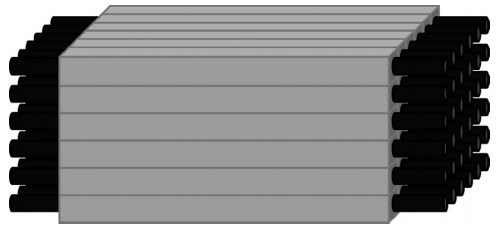
\includegraphics[width=\linewidth]{Chapter2/Figs/Raster/Panda_far.png}
  \captionsetup{width=.9\linewidth}
  \caption{The exterior of PANDA. The bars are clustered together with photon multiplier tubes at the end to measure photons.}
  \label{subFig:pandaFar}
\end{subfigure}%
\begin{subfigure}{.5\textwidth}
  \centering
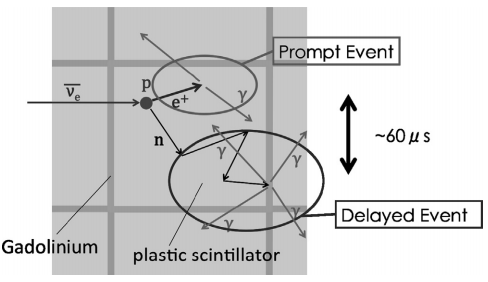
\includegraphics[width=\linewidth]{Chapter2/Figs/Raster/Panda_close.png}
  \captionsetup{width=.9\linewidth}
  \caption{Interior of the PANDA detector, prompt event of a positron and delayed gadolinium capture and cascade from a neutron event.}
  \label{subFig:pandaClose}
\end{subfigure}
\caption{Exterior (\ref{subFig:pandaFar}) and interior (\ref{subFig:pandaClose}) of the PANDA detector. From \cite{PANDA_2014}.}
\label{fig:pandaCloseFar}
\end{figure}

The bars are not positioned perpendicularly in the $z$ direction (figure \ref{subFig:pandaFar}). Therefore tracking is more difficult in PANDA, due to not having specific $x$ and $y$ coordinates, this makes vetoing cosmic $\mu$ (a major source of background) potentially harder in PANDA than if the bars were perpendicular. The photon multiplier tubes (PMTs) used in PANDA are also expensive, the PANDA36 shown in figure \ref{subFig:pandaFar} is much smaller than the proposed final design of 100 channels and 1m$^3$ \cite{PANDA_2012} but PANDA is being built in stages because of the expense of these components. However, the potential for measuring many photons with high efficiency makes PMTs attractive. Both Lesser PANDA (16 channels) and PANDA36 have been deployed by van with background measurements and reactor measurements being taken from inside the van \cite{PANDA_2012}, \cite{PANDA_2014}. But due to the flammable nature of petrol and diesel, it is unclear whether reactor operators would be open to having a van stationed indefinitely outside their reactor buildings. PANADA36 has also been used for monitoring Terrestrial $\gamma$-ray Flashes (TGFs) from thunderstorms to allow for further background reduction at nuclear sites\cite{PANDA_tgf}. 
\\\\The SoLid detector is a plastic scintillating detector that uses wavelength shifting (WLS) fibres with MPPCs at the end to read out fibre signals and adjacent 5\,cm $\times$ 5\,cm $\times$ 5\,cm cubes being lit up at similar time intervals to discern particles \cite{Solid_proposal}. There is a prompt signal outputted from the positron in the plastic cubes and a delayed signal from the $^6$LiF:ZnS(Ag) screen interacting with neutrons as shown in figure \ref{fig:SolidCubeDiagram}. The prompt positron response and delayed neutron response is similar to the other experiments mentioned. In SoLid $^6$Li is used as the neutron capture agent (equation \ref{Li_interact_eq}), which produces an $\alpha$ and a 4.78\,MeV $\gamma$ \cite{Solid_readout}. The $\gamma$ signal is ignored because the $\alpha$ signal produced is clear and produces a specific pulse shape signal \cite{Solid_readout} which has a very minimal background due to its specific pulse shape. Setting it apart from other experiments that use the 8\,MeV Gd cascade. 

\begin{equation}
n + {^6Li} \rightarrow {^3H} + \alpha +4.78\,MeV
\label{Li_interact_eq}
\end{equation}

\begin{figure}[htbp]
 \centering
 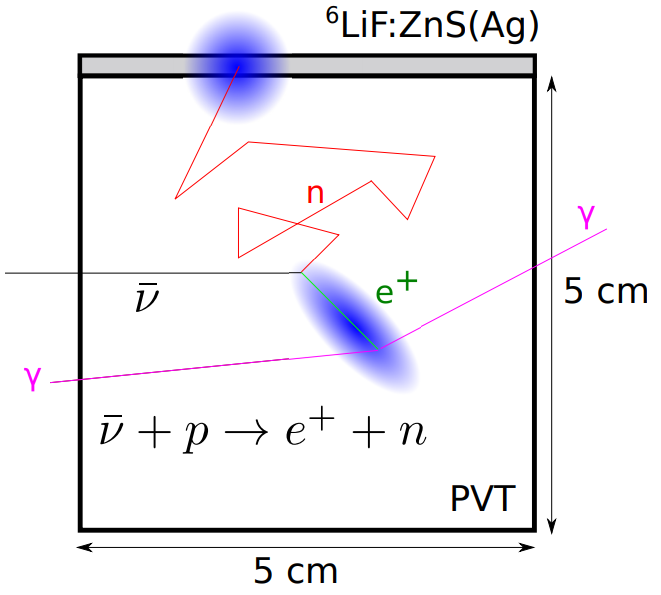
\includegraphics[height=58mm]{Chapter2/Figs/Raster/SoLid_cube.png}
 \captionof{figure}{SoLid cube during an inverse beta decay event anti-neutrino decays into a positron and neutron via equation \ref{inverse_beta_decay}, delayed neutron is captured by $^6$LiF:ZnS(Ag) screen, positron gives the prompt response. From \cite{Solid_readout}.} 
 \label{fig:SolidCubeDiagram}
\end{figure}

The challenge with using $^6$Li as a neutron capture agent is producing enough light for pulse shape discrimination (PSD) to be used in the analysis. The $\alpha$s need to be captured by the sulphur in the $^6$LiF:ZnS(Ag) screen which then emits a specific $\gamma$ into the plastic which in turn produces electrons via Compton scattering which are then captured by WLS fibres. The Wavelength shifting fibres may not capture enough photons for the pulse shape analysis to be used, an alternative method to this is that proposed by CHANDLER (Carbon Hydrogen Anti-Neutrino Detector with a Lithium Enhanced Raghavan-optical-lattice) \cite{aap2015}. Which uses PMT's and a Raghavan-optical-lattice to counter-act the low light issues in SoLid. However, the CHANDLER design also brings challenges as the detector cannot be too large otherwise attenuation and containment of events prevent signals from being read. 

\section{Background At Reactor Sites}
The PROSPECT experiment has done a  study looking into the background at two research reactor locations difference between the National Bureau of Standards Reactor (NBSR) at NIST and the High Flux Isotope Reactor (HFIR) at ORNL \cite{Ashenfelter_2016}. Another site was considered by the PROSPECT the ATR at INL but the increased altitude of that site leads to a significantly higher cosmogenic neutron flux \cite{Ashenfelter_2016}. An example of how reactors affect the background can be seen in figure \ref{fig:Prospect_NSBR_gammaSpec} which shows how the $\gamma$ spectrum varies when the NBSR is on and off, it shows how the spectrum between 3\,MeV -- 9\,MeV is mostly dominated by reactor noise. Another component is neutron measurements caused by the reactor which is shown in figure \ref{fig:prospectNeutronMap} for thermal neutrons which are an issue for $\bar{\nu_e}$ detectors but should be somewhat negated through robust e$^+$ identification and accurate double coincident measurements. Another more important background is fast neutrons because they cause a false double coincident signal by potentially interacting with protons and then thermalising and being absorbed. The measurement of cosmogenic neutron background has been done by JEDEC in 2006 \cite{JEDEC_2006} as well as PROSPECT in figure \ref{fig:Prospect_HFIR_NBSR_nearFarPlots} which shows similar rates at different locations this is unsurprising as this is largely a function of altitude more than any other factor \cite{Ashenfelter_2016}. However, a certain type of background that is easy to mitigate (for VIDARR) but also extremely useful is the cosmic $\mu$ background. Cosmic $\mu$ have a large number of events of $\sim$ 119\,s$^{-1}$m$^{-2}$ according to the CRY library \cite{ieee_cry_2007} (also see figure \ref{fig:CRY_rates}). These particles can be detected by very simple detector requiring only a series of paddles as seen in figure \ref{fig:Prospect_MuonPaddels} done by PROSPECT. This cosmic $\mu$ background is useful as they are highly penetrating particles tracks that can be approximated to be straight lines (later discussed in chapter \ref{chp:cosmicMuonTomography}). The range of angles incident cosmic $\mu$ posses make them useful for tomographic purposes as will be discussed in section \ref{sec:cosmicMuTelescopes}. % The angles of incidence of cosmic $\mu$ can have many useful applications and as such these cosmic $\mu$ should not be excluded as mere noise as will be shown in section \ref{sec:cosmicMuTelescopes}.

\begin{figure}[htbp]
 \centering
 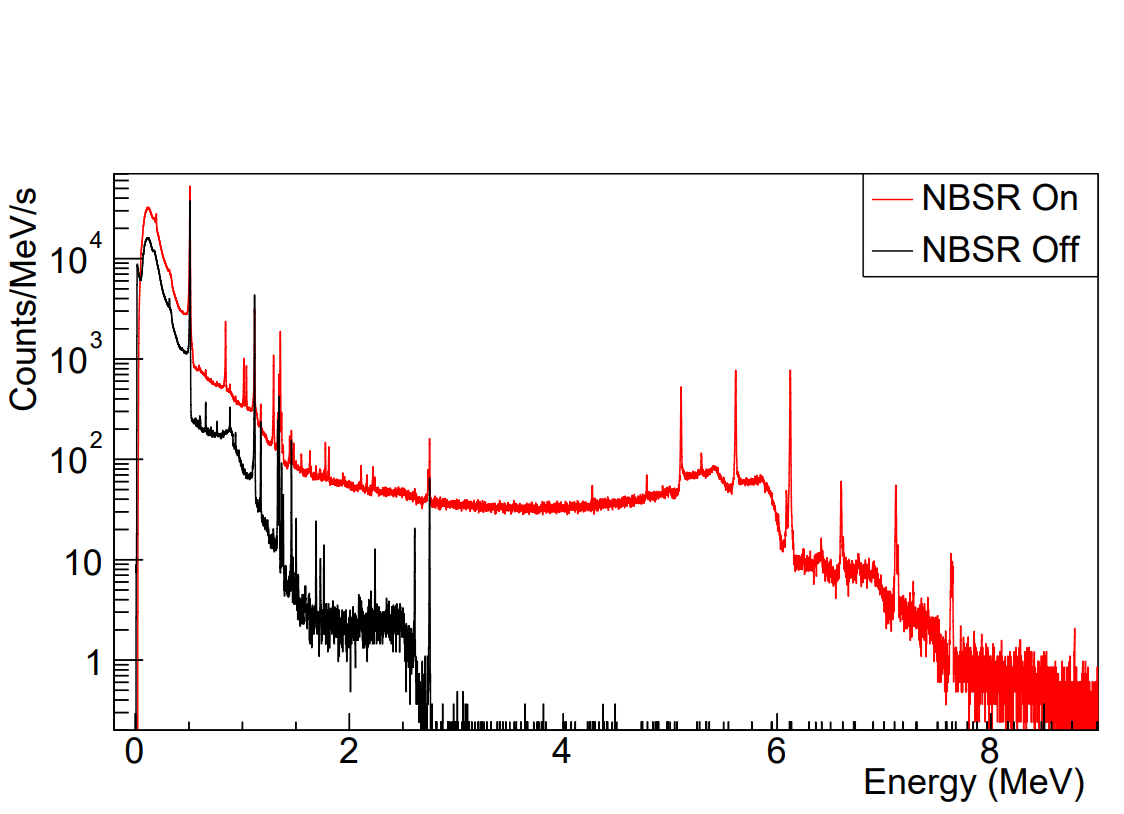
\includegraphics[width=0.7\linewidth]{Chapter2/Figs/Raster/Prospect_NSBR_gammaSpec.png}
 \captionof{figure}{Example HPGe $\gamma$-ray spectra taken with the NBSR on and off. Prominent lines, and associated escape peaks and Compton continua, are evident. From \cite{Ashenfelter_2016} (table 2 in \cite{Ashenfelter_2016} shows line sources).} 
 \label{fig:Prospect_NSBR_gammaSpec}
\end{figure}

\begin{figure}[htbp]
 \centering
 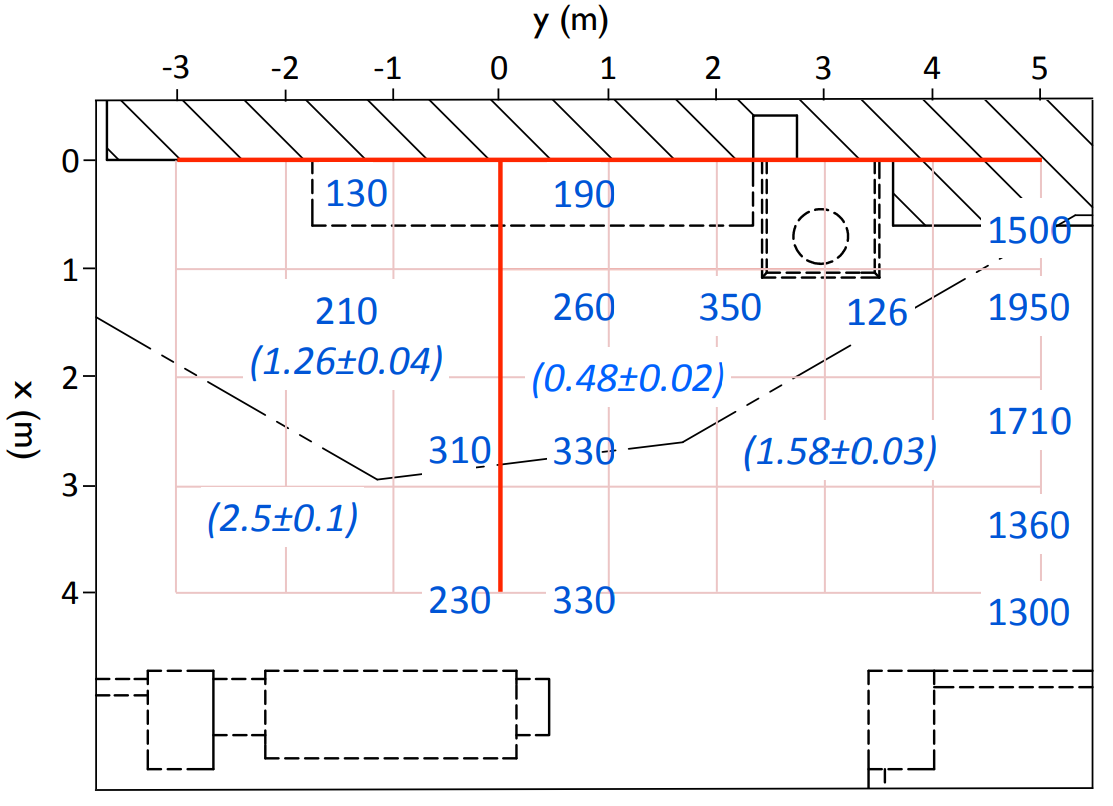
\includegraphics[width=0.7\linewidth]{Chapter2/Figs/Raster/prospectNeutronMap.png}
 \captionof{figure}{A pictorial representation of neutron dose rates (measured in nSv/h) and thermal neutron rates in italics (cm$^{-2}$ s${^-1}$) at the HFIR near location roughly 15\,cm (z = 0.15) above the floor. Measurements are plotted on a one meter square grid refernced to the ractor wall (x = 0) and the smallest baseline (y = 0). The reactor core is centred at (x,y,z) = (-4.06,0,-3.85). From \cite{Ashenfelter_2016} } 
 \label{fig:prospectNeutronMap}
\end{figure}

% \begin{figure}[htbp]
%  \centering
%  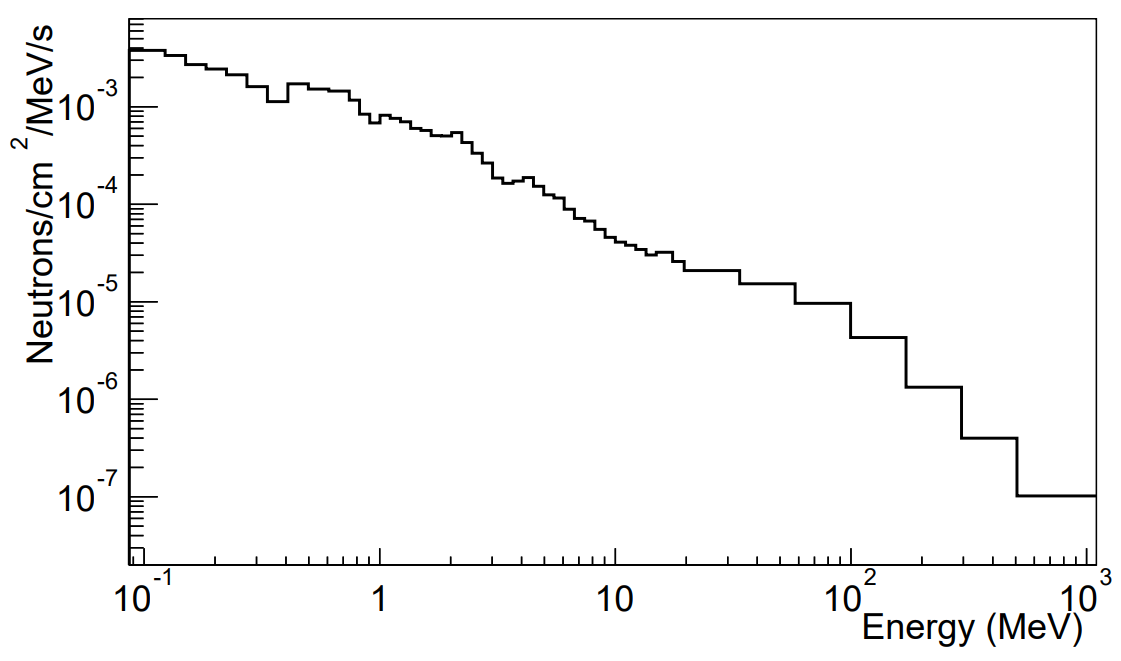
\includegraphics[width=0.7\linewidth]{Chapter2/Figs/Raster/JDEC_neutronSpec.png}
%  \captionof{figure}{The JEDEC standard fast neutron spectrum recorded at sea
% level in New York. From \cite{JEDEC_2006}. } 
%  \label{fig:JDEC_neutronSpec}
% \end{figure}

\begin{figure}[htbp]
\centering
\begin{subfigure}{.5\textwidth}
  \centering
  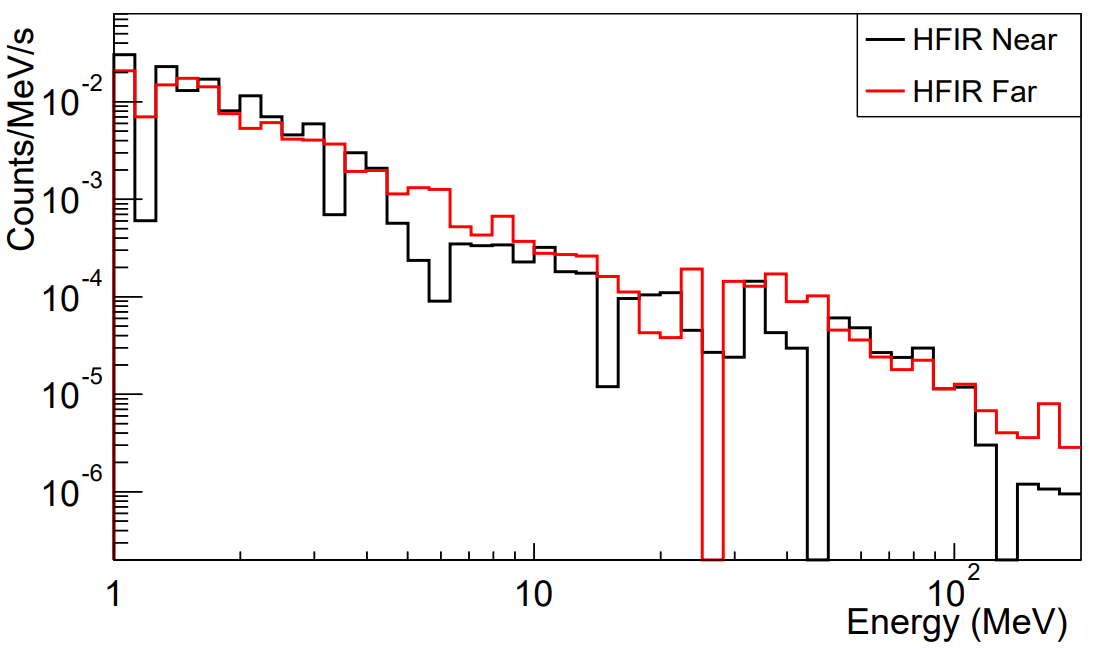
\includegraphics[width=\linewidth]{Chapter2/Figs/Raster/Prospect_HFIR_nearFarPlot.png}
  \captionsetup{width=.9\linewidth}
  \caption{}
  \label{subFig:Prospect_HFIR_nearFarPlot}
\end{subfigure}%
\begin{subfigure}{.5\textwidth}
  \centering
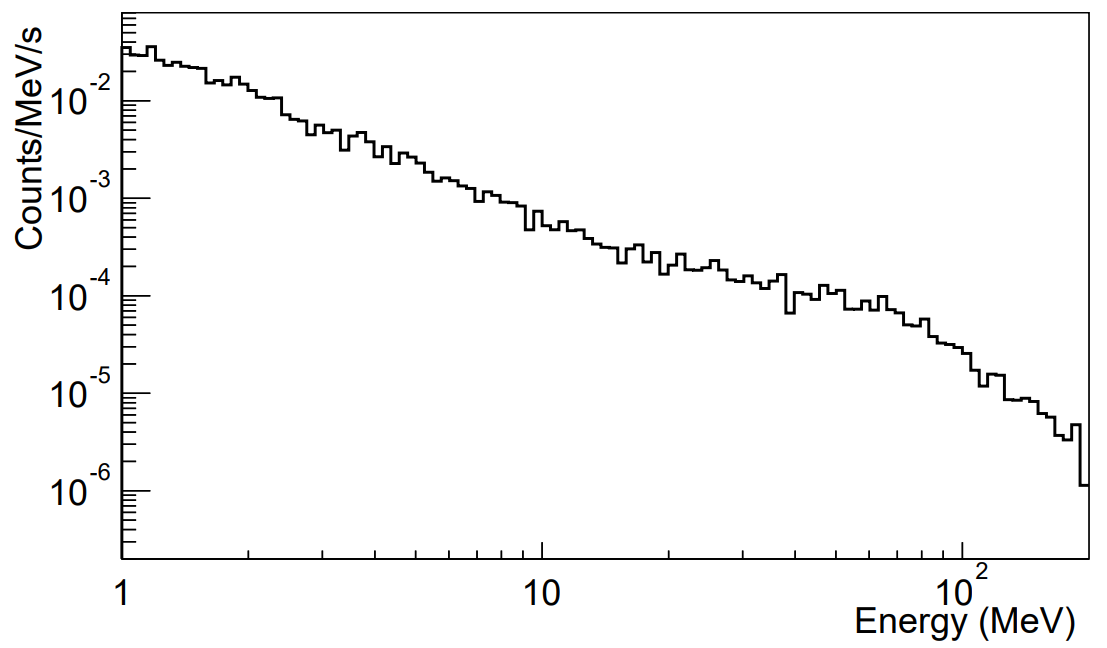
\includegraphics[width=\linewidth]{Chapter2/Figs/Raster/Prospect_NBSR_farPlot.png}
  \captionsetup{width=.9\linewidth}
  \caption{}
  \label{subFig:Prospect_NBSR_farPlot}
\end{subfigure}
\caption{The cosmogenic neutron-induced energy spectrum was recorded at the (a) HFIR near and far locations and (b) NBSR far location. From \cite{Ashenfelter_2016}.}
\label{fig:Prospect_HFIR_NBSR_nearFarPlots}
\end{figure}

\begin{figure}[htbp]
 \centering
 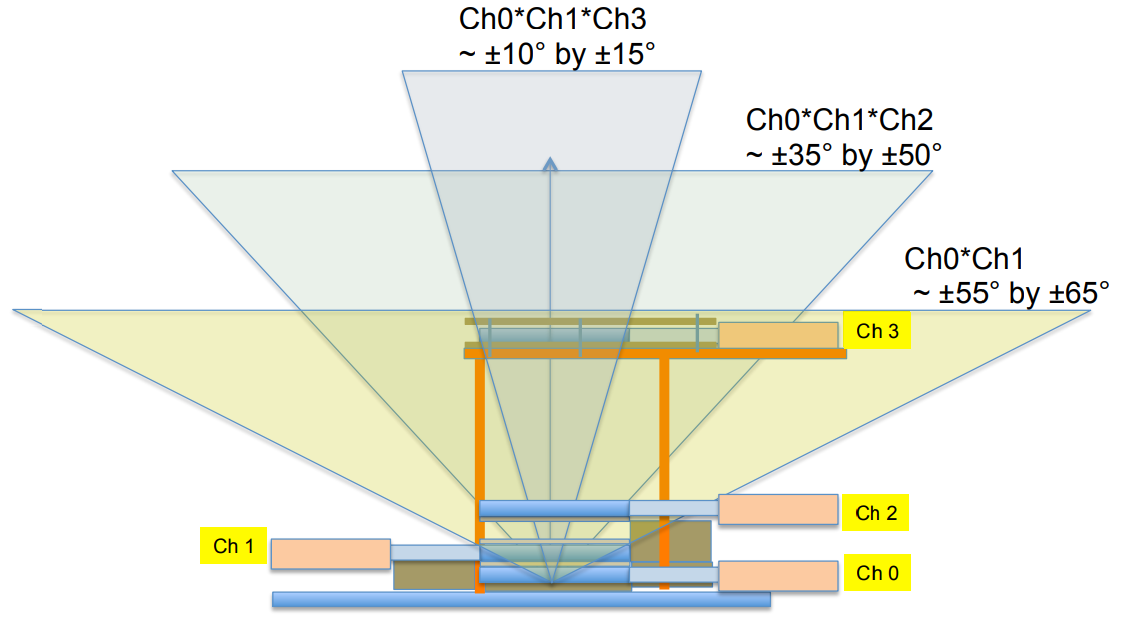
\includegraphics[width=0.7\linewidth]{Chapter2/Figs/Raster/Prospect_MuonPaddels.png}
 \captionof{figure}{The angular acceptances for the $\mu$ telescope instrument
used at all sites is determined by the coincidence requirement enforced
between the 4 plastic scintillator paddles. From \cite{Ashenfelter_2016}.} 
 \label{fig:Prospect_MuonPaddels}
\end{figure}

\section{Cosmic $\mu$ Telescopes} \label{sec:cosmicMuTelescopes}
Both DIAPHANE and MU-RAY have taken tomographic data to image their surroundings. With DIAPHANE imaging La Soufriere of Guadeloupe using cosmic $\mu$ radiography as seen in figure \ref{fig:diaphaneStructualImaging} which shows the different density areas of rock relevant for volcanology \cite{Marteau_2017}.  MU-RAY has also produced similar results for mt. Vesuvius in figure \ref{fig:mtVesuviusMuRayImaging}. Though their technique and data only provide results of rock thickness in meters rather than density \cite{Ambrosino_2014}. Of more interest is figure \ref{fig:mtVesuviusMuRayTransmission} from MU-RAY which shows the ``Transmission'' method. The transmission method used in figure \ref{fig:mtVesuviusMuRayTransmission} is obtained by pointing the MU-RAY detector at the sky for a calibration period of one week then pointing the MU-RAY detector at Mt Vesuvius for one week and then taking the ratio of the two data sets \cite{Ambrosino_2014}. This approach of measuring the free sky and the blocked sky and taking the ratio of the two creates an extremely clear image because it takes the background into account. This creates a clear difference in intensity where transmission of 1 represents the free sky and transmission of 0 represents completely blocked sky. This approach is the one that will be used when analysing the Wylfa reactor site (see chapter \ref{chp:cosmicMuonTomography}) due to the effective reduction of background noise effects and the sharpness of the image it provides. 
\\\\The DIAPHANE experimental setup seen in figure \ref{fig:DIAPHANE_deployment} shows a cosmic $\mu$ telescope with several different planes clearly analysing a very narrow field of view this helps significantly in preventing distortions via bin migration. This is also the case for the MU-RAY collaboration as seen in figure \ref{fig:muRayDetectors} the detector is also multiple flat planes. Each plane in MU-RAY is compromised of triangular prisms with WLS fibres running down the middle (see figure \ref{fig:muRaySetup}). Both MU-RAY and DIAPHANE are traditional cosmic $\mu$ telescopes as opposed to VIDARR which is an $\Bar{\nu_e}$ detector first and a cosmic $\mu$ camera second. Despite this DIAPHANE, MU-RAY, and VIDARR all use similar technology: plastic scintillating bars and WLS fibres \cite{Carroll_2018} \cite{Marteau_2017} \cite{ANASTASIO2013423}. DIAPHANE uses ``multianode PMT’s'' to read out information from the WLS fibres \cite{Marteau_2017} whereas VIDARR and MU-RAY use SiPms \cite{Carroll_2018} \cite{ANASTASIO2013423} to read out the information from the WLS fibres. 

\begin{figure}[htbp]
 \centering
 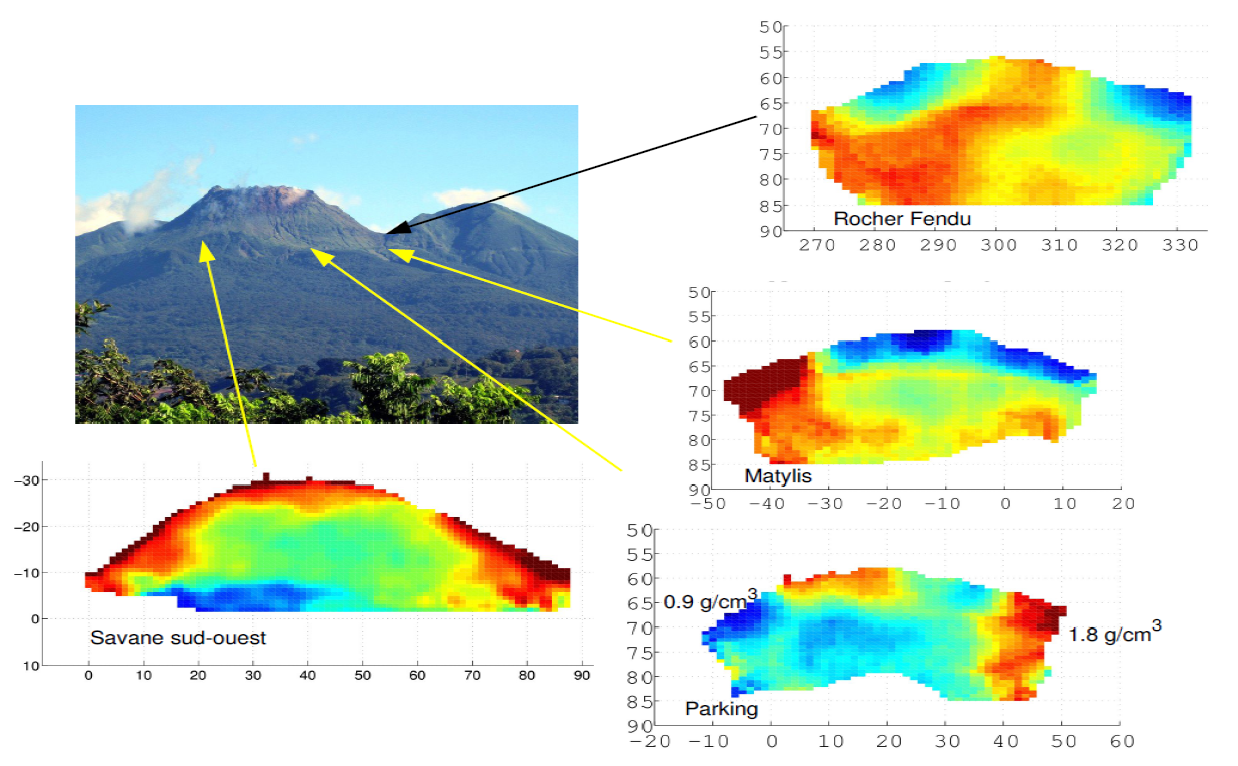
\includegraphics[width=1.0\linewidth]{Chapter5/Figs/Raster/diaphane_structuralImaging.png}
 \captionof{figure}{DIAPHANE structural imaging of the La Soufriere of Guadeloupe dome from 4 different acquisition sites around the dome. The blue areas are the less dense zones of the volcano. The red areas have the highest density. The average density extracted from all those images ranges from 1.6 to 1.8 g.cm$^{-3}$. From \cite{Marteau_2017}} 
 \label{fig:diaphaneStructualImaging}
\end{figure}

\begin{figure}[htbp]
 \centering
 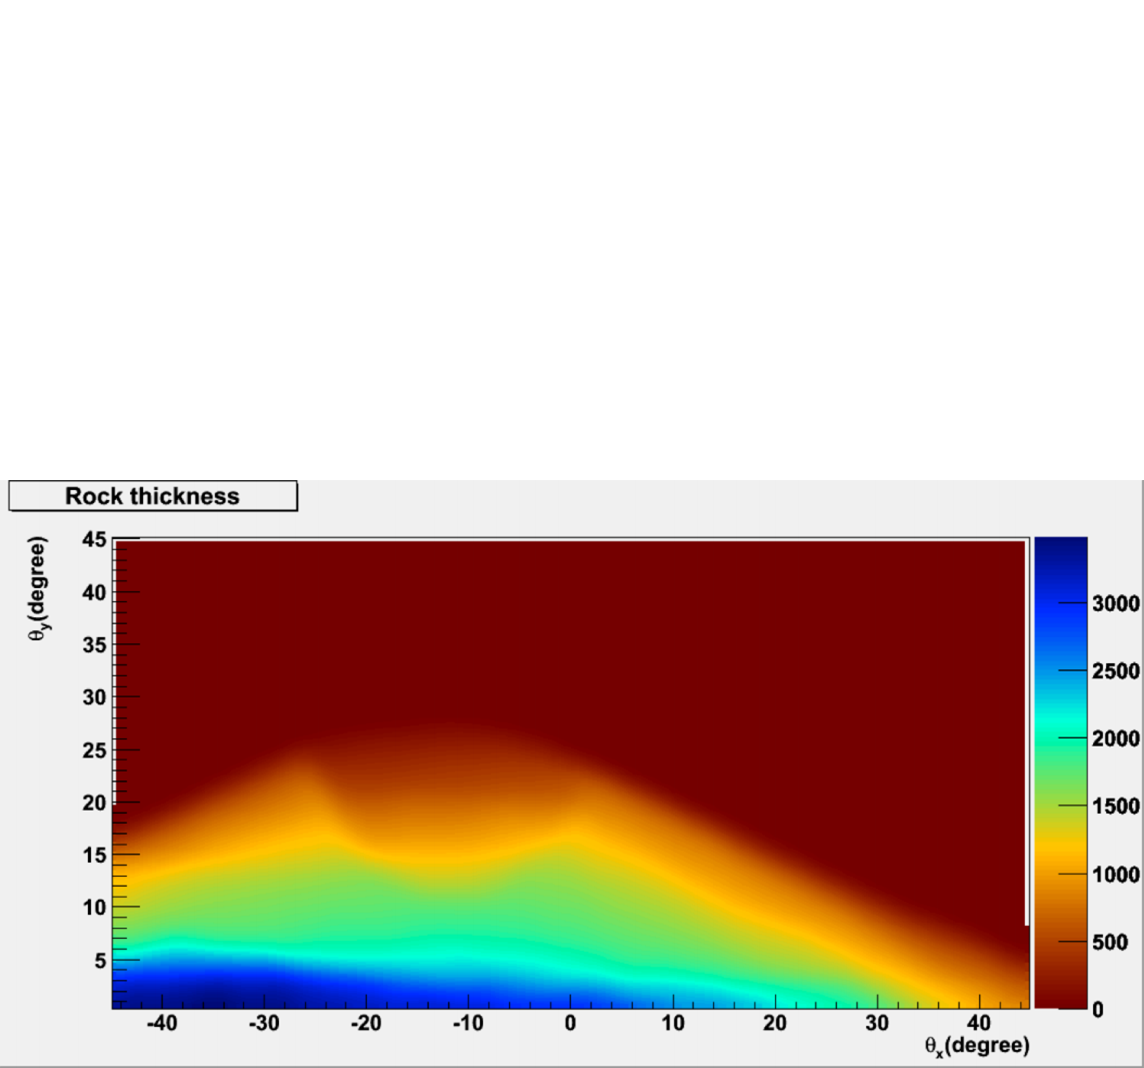
\includegraphics[width=0.7\linewidth]{Chapter5/Figs/Raster/mtVesuviusMuRayImaging.png}
 \captionof{figure}{MU-RAY telescope analysing Vesuvius rock thickness, expressed in m, as seen from the observation point at $\sim$ 800 m altitude. From \cite{Ambrosino_2014}.} 
 \label{fig:mtVesuviusMuRayImaging}
\end{figure}

\begin{figure}[htbp]
 \centering
 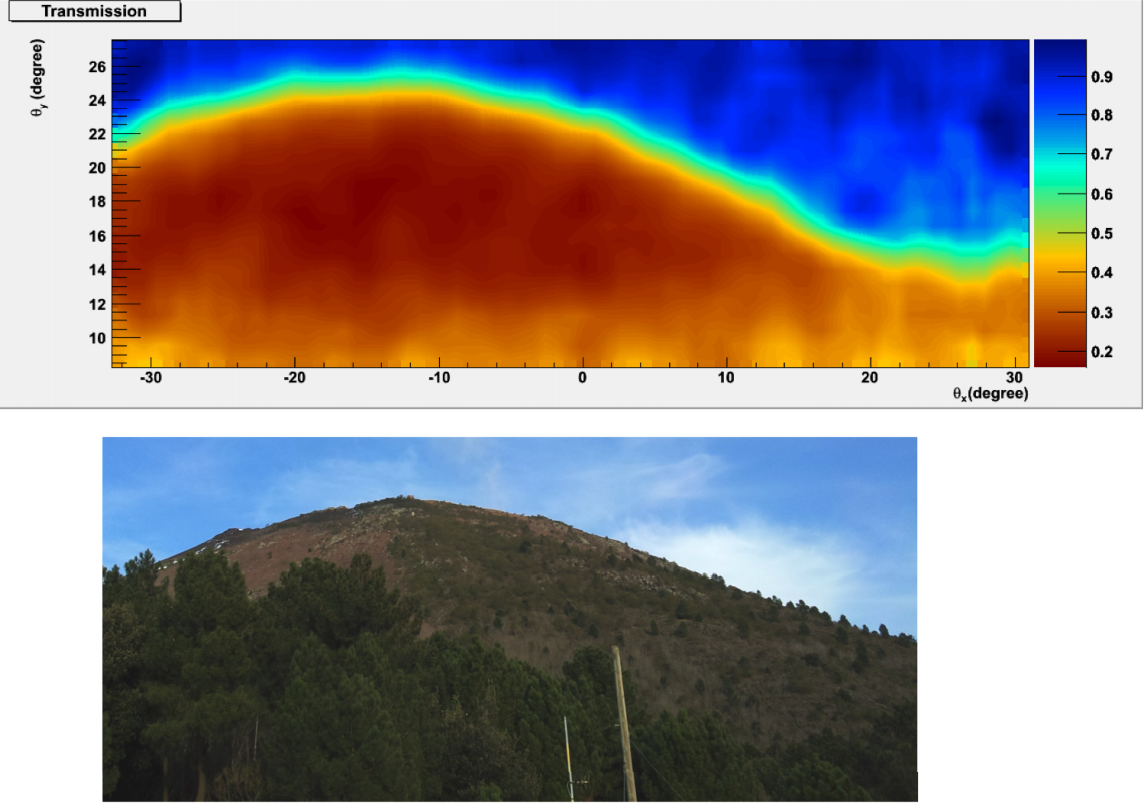
\includegraphics[width=1.0\linewidth]{Chapter5/Figs/Raster/mtVesuviusMuRayTransmission.png}
 \captionof{figure}{MU-RAY data from Vesuvius. Top: the transmission histogram of Mt Vesuvius after one week of data taking. Bottom: a picture of Mt Vesuvius taken by the telescope observation point. From  \cite{Ambrosino_2014}.} 
 \label{fig:mtVesuviusMuRayTransmission}
\end{figure}

\begin{figure}[htbp]
 \centering
 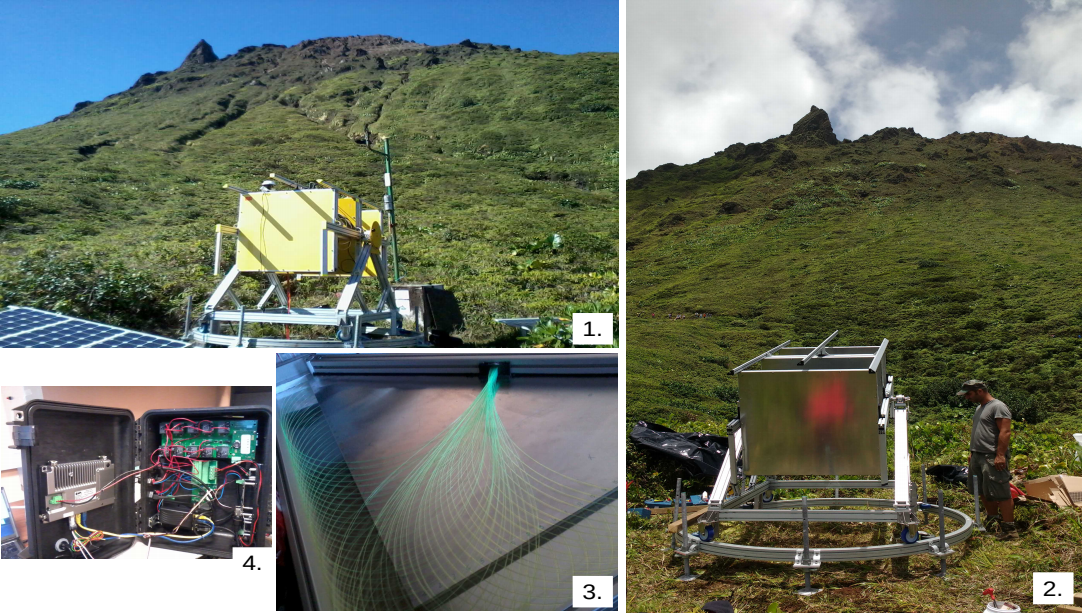
\includegraphics[width=1.0\linewidth]{Chapter5/Figs/Raster/DIAPHANE_deployment.png}
 \captionof{figure}{The deployment of the DIAPHANE detector from \cite{Marteau_2017}. DIAPHANE $\mu$ detectors upgrades. 1: the first generation 3 planes $\mu$ detector on the slope of La Soufrière of Guadeloupe (PK site). 2: the second-generation 3 planes $\mu$ detector, with a transverse segmentation divided by a factor 2, on the slope of La Soufrière of Guadeloupe (SAM site). 3: inner WLS fibres collected on a PMT cookie. 4: compact CTRL BOX with embedded hardened processing unit and electronics: common clock signal, WebRelay, Ethernet switch, Power-over-Ethernet to the wifi antenna. From \cite{Marteau_2017}.} 
 \label{fig:DIAPHANE_deployment}
\end{figure}

\begin{figure}[htbp]
 \centering
 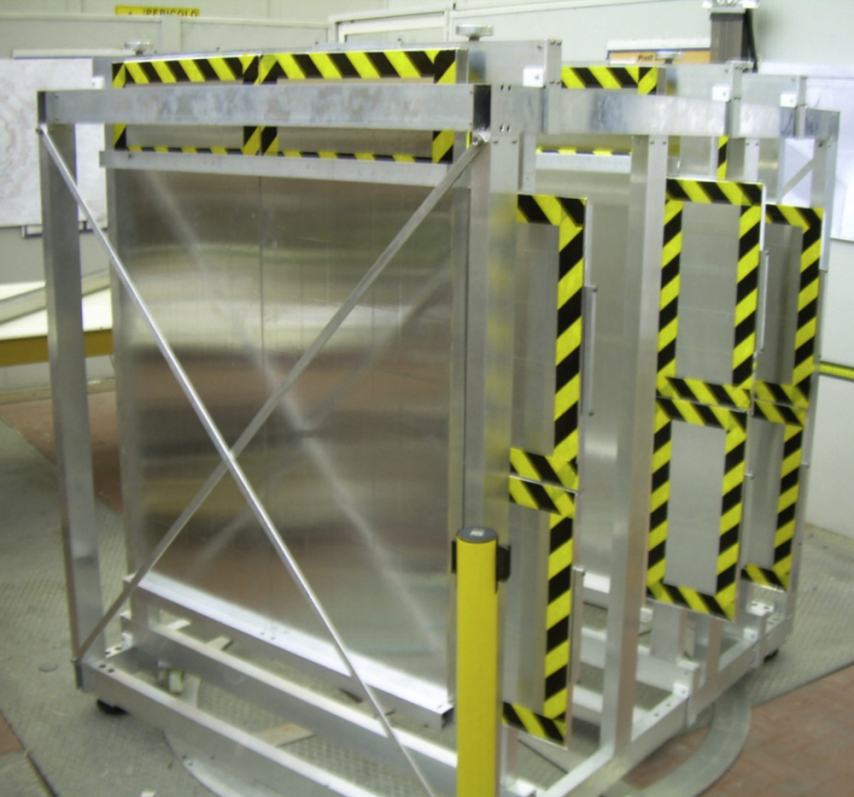
\includegraphics[width=0.7\linewidth]{Chapter5/Figs/Raster/muRayDetectors.png}
 \captionof{figure}{The MU-RAY detector frame with the three X–Y planes mounted. The frame can be oriented using the rotating platform visible at the bottom. From \cite{ANASTASIO2013423}} 
 \label{fig:muRayDetectors}
\end{figure}

\begin{figure}[htbp]
 \centering
 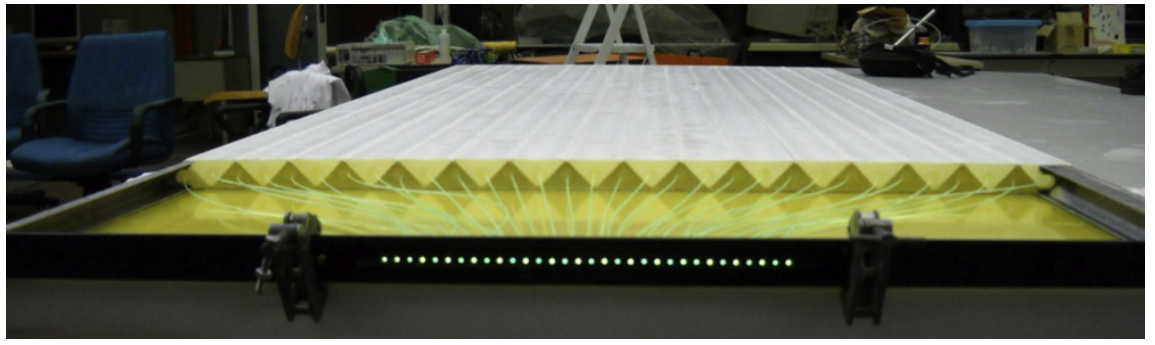
\includegraphics[width=0.7\linewidth]{Chapter5/Figs/Raster/muRaySetup.png}
 \captionof{figure}{The scintillator for the MU-RAY collaboration, unlike VIDARR they use a triangular prism-shaped scintillator. From \cite{ANASTASIO2013423}.} 
 \label{fig:muRaySetup}
\end{figure}
